\documentclass{article}

\usepackage[margin=1in]{geometry}
\usepackage{graphicx} 
\usepackage{gensymb}
\usepackage{amsmath}
\usepackage{multicol}
\usepackage[font=small,labelfont=bf]{caption}

\title{How the Scalar works}

\begin{document}
\begin{center}
    {\huge{How the Scalar function works}}
\end{center}    
    \begin{multicols}{2}
    The main problem of the data generated by the model is the scale of the data itself.
    As we can see in the following picture, the serie seems realistic if we just look at the trend.
    However, the magnitude of the data is totally out of scale. The algorithm below is designed to force
    the series to converge to the real data range.
    \subsection*{Introduction}
    The scaler aims at scaling the time serie without affecting the trend. The idea is that when we have 
    a peak of returns in the time serie, the significance of the peak depends on its distance from the second highest peak in the serie. For exemple let's take the following series from the dataset of stock values:\\
    \begin{center}
        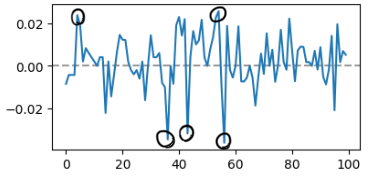
\includegraphics[scale = 0.7]{imgs/small_peaks.png}
        \captionof{figure}{}
        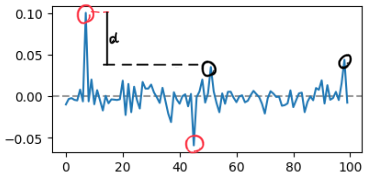
\includegraphics[scale = 0.7]{imgs/big_peaks.png}\\
        \captionof{figure}{}
    \end{center}
    As we can see the in (\textbf{Figure 1}) the 2 highest peaks are not very far from each other and that makes the order of magnitude lower compared to the peak we can see in the (\textbf{Figure 2}). Let's analyze two different meanings a peak can refer to:
    \begin{itemize}
        \item a strong movement in price
        \item a shock, due to news or particural events.
    \end{itemize}  
    Taking into consideration the nature of the sample taken, it is very unlikely to have two big shocks in the same window. Following this logic, when the $1^{st}$ and $2^{nd}$ peaks in a serie are close, we can conclude they are probably just strong movements in the price. Again, when the $1^{st}$ peak in terms of magnitude is way bigger than the $2^{nd}$, it is unlinkely to have price movements with this elevated magnitude, in very small ranges. We can note that since the usual price movement of these kind of stocks falls between a range of -0.01\% and 0.01\%, It seems reasonable to apply the scalar function to get an ultimate generated serie that can be used for data analysis purposes while reflecting the true nature of the financial asset. 
    \subsection*{Scalar Logic}
    Baset on the above reasonment the Scalar aims assign to "lonley" peaks in the generated series the value that usually shocks have in the real data 
    and assign to close peacks value that are typical of strong market movements.
    \subsection*{Scalar Implementation}
    To do It the scalar compute the quantiles of the max values distribution and same thing for the distribution of the difference between the $1^{st}$ and 
    $2^{nd}$ peaks.\\
    Then the algorith take the sample and see where the distance between the $1^{st}$ and $2^{nd}$ peaks are among the quantiles of the differences for real 
    data. Then pick a random value from a uniform distribution where the lower and upper bonudaries are the corresponding quantiles in the max distribution. 
    Same thing for the negative peaks.
    \end{multicols}
    \textbf{Exemple:}
    \begin{center}
        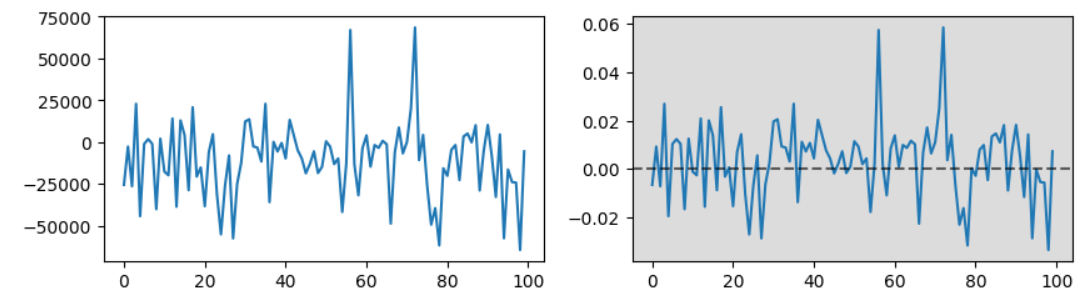
\includegraphics[scale=0.6]{imgs/EX_03.png}
    \end{center}
    In the above exemple we can see on the left the series generated by our model and on the rigth the series after the we apply the Scaler. As we can see 
    the scaler preserves the pattern generated by our model and just rescale the data so we have realistic data.
\end{document}
